\section{Results}
\label{sec:results}

This section reports, one question at a time, what each experiment shows. Unless a heading says otherwise, a score is
test macro-F1 (\%, mean $\pm$ SD over the five rounds) on the session-blocked split, and ``photos'' are test photos.

\subsection{Controls that never see the leaf}
\PaperTable[\ColumnLayout]{shortcuts}{Controls that never see the leaf: test macro-F1 and balanced accuracy (\%), mean $\pm$ SD over the 5 rounds, on the locked and on the session-blocked split. ``Time neighbour'' predicts the class of the nearest training photo in time from the same camera; ``strict'' keeps only paper-coloured pixels outside the grown leaf mask.}

Table~\ref{tab:final_shortcuts} shows how far acquisition cues alone go. Guessing by class share scores 25.2 macro-F1 and
the majority class 15.4. Colour alone (43.5 $\pm$ 2.8) and the Otsu-derived background alone (39.7 $\pm$ 3.6) are above
that on the session-blocked split, so some signal sits outside the lesions; a stricter mask that keeps fewer leaf pixels gives 38.9 $\pm$ 4.9. The nearest-in-time baseline, which never sees the image, scores 80.5 $\pm$ 1.6 on the locked split and
30.4 $\pm$ 10.8 on the session-blocked split. On the locked split a score near 80 therefore does not show that a
model recognises disease, and we use the session-blocked split as the headline.

\subsection{Tiles against whole-image models (H1, H2)}
\PaperTable[\SmallWide]{main}{Main results: test macro-F1 and balanced accuracy (\%), mean $\pm$ SD over the 5 rounds. Session: session-blocked split, the headline (each method tuned on its own validation photos, its selected configuration tested once; ConvNeXt-T at 448 px keeps the learning rate chosen at 224 px). Locked: the locked split. Paddy: zero-shot scores on 8{,}086 Paddy Doctor photos at native zoom, and macro-F1 at the other two zoom levels for the tile methods; nothing was trained or tuned on them.}

\PaperTable[\SmallWide]{paired_session}{Attention MIL (A) against every other method, session-blocked test photos. Difference of the pooled scores in points (A minus the other; it can differ from the difference of the round means), 95\,\% photo and block ranges, rounds won by A, and the verdict under each range (rule in Section~\ref{sec:setup:metrics}).}

Table~\ref{tab:final_main} gives the main results and Table~\ref{tab:final_paired-session} the paired tests.
Attention MIL scores 77.9 $\pm$ 3.1, ahead of Swin-T (76.3 $\pm$ 4.1), ConvNeXt-T at 224 px (75.0 $\pm$ 5.0),
EfficientNetV2-S (74.1 $\pm$ 4.8) and InceptionV3 (72.0 $\pm$ 3.6) in mean. Under both ranges and in 5 of 5 rounds it
beats InceptionV3 (+5.9), EfficientNetV2-S (+2.9), both linear probes (+4.6, +3.1), Mean pooling over tiles (+7.2), Max pooling
over tiles (+3.0) and both whole-photo controls (+8.0 at 224 px, +3.9 at 512 px). Against ConvNeXt-T at 224 px it beats
under the photo range only (+2.8; block range $[-0.1, +6.1]$), and against Swin-T there is no clear difference on
macro-F1 (+1.4), although there is on balanced accuracy (+2.0). Max pooling is not clearly different on balanced accuracy.
H1 is therefore supported on this split: with the same head and encoder, tiles at a common leaf scale beat one
whole-photo description. H2 is supported against mean pooling and, on macro-F1, against max pooling.
On the locked split (Table~\ref{tab:final_paired-locked}) Attention MIL scores 82.8 $\pm$ 1.5 and is not clearly different
from any whole-image model; it beats Mean pooling over tiles (+4.4) and the 224-px whole-photo control (+2.7),
and there is no clear difference against the 512-px control on macro-F1 (+1.1).

ConvNeXt-T at 448 px scores 79.2 $\pm$ 3.8, above the mean of Attention MIL. Attention MIL minus ConvNeXt-T (448 px) is
$-1.5$ (photo range $[-3.0, +0.2]$, block range $[-3.3, +0.9]$), with Attention MIL winning 1 of 5 rounds: no clear
difference. This test was declared after both means were seen. We make no claim that either is better.

\subsection{Resolution, Otsu preprocessing and pixel scale}
\PaperTable[\SmallWide]{conditions}{Whole-image models at other input conditions: test macro-F1 and balanced accuracy (\%), mean $\pm$ SD over the 5 rounds, session-blocked split. The learning rate chosen at 224 px was kept.}

\PaperTable[\SmallWide]{ablations_test}{The two tile variants tested once on the session-blocked test photos: score (\%, mean $\pm$ SD over 5 rounds) and the difference of the pooled scores, main (Attention MIL) minus variant, in points (so it can differ from the difference of the means). \texttt{otsu\_on}: tiles of Otsu-cleaned photos; \texttt{native\_scale}: tiles at the stored resolution.}

Table~\ref{tab:final_conditions} shows the whole-image models at other conditions. At 128 px every model falls (56.9--67.8,
against 72.0--76.3 at 224 px); ConvNeXt-T at 448 px rises to 79.2. Otsu preprocessing at 224 px helps none of the four
(70.2--73.5). Attention MIL beats all eight of the 128-px and Otsu conditions under both ranges and both metrics in 5 of 5
rounds (Table~\ref{tab:final_paired-conditions}); these tests were declared after the means were seen. The two tile ablations
tested on the test photos (Table~\ref{tab:final_ablations-test}) agree: Attention MIL beats tiles of Otsu-cleaned photos
(+5.2) and tiles at the stored, native scale (+2.9; 4 of 5 rounds) under both ranges. The remaining ablations
were scored on validation photos only (Table~\ref{tab:final_ablations}), where the main configuration is favoured because its
settings were chosen there. A supervised ConvNeXt-T encoder scores 66.5 against 78.5, DINOv2-B 76.1 and the smaller
DINOv3 ViT-S/16 74.8; 448-px tiles shrunk to 224 px (77.8), an unweighted loss (77.9) and the class token alone (77.5) are
within the 1.4-point change seen when the same configuration is trained with other seeds (77.1).

\subsection{A committee of two}
\PaperTable[\SmallWide]{paired_committee}{Committee against ConvNeXt-T (448 px) alone, session-blocked test photos: difference of the pooled scores in points (committee minus ConvNeXt-T). Declared after both means were seen; ConvNeXt-T is a member of the committee, so the two are not independent.}

A Committee of ConvNeXt-T (448 px) and Attention MIL scores 81.6 $\pm$ 3.6 (balanced accuracy 81.4 $\pm$ 4.5). Both
members were chosen on validation photos and the Committee was tested once. It beats Attention MIL under both ranges (+3.6,
5 of 5 rounds), as declared in advance. It also beats ConvNeXt-T (448 px) alone (Table~\ref{tab:final_paired-committee}:
+2.2, 4 of 5 rounds, both ranges); this second test was declared after the means were seen, and ConvNeXt-T is one of the
two members, so the two comparisons are not independent. The Committee is less well calibrated (ECE 0.102 against 0.050
for ConvNeXt-T alone) and scores lower than Attention MIL on Paddy Doctor (23.0 against 26.1). A Committee of the two whole-image models
ConvNeXt-T (448 px) and Swin-T scores 80.3 $\pm$ 4.0 and also beats Attention MIL (+2.5, 5 of 5 rounds, both ranges).

\subsection{Which classes fail}
\PaperTable[\SmallWide]{per_class}{Per-class recall (\%) on the session-blocked test photos, pooled over the 5 rounds (every test photo once). Hispa is the pre-declared diagnostic class. Last row: number of test photos per class.}

\begin{figure*}[t]
\centering
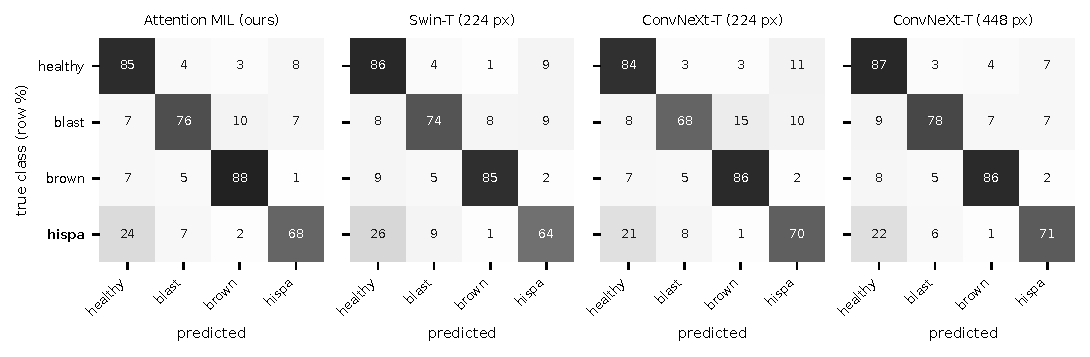
\includegraphics[width=0.8\textwidth]{final_confusion.pdf}
\caption{Row-normalised confusion matrices (\% of the true class) of four methods on the session-blocked test photos, pooled over the 5 rounds. The bold row is hispa, the pre-declared diagnostic class; counts are in Table~\ref{tab:final_confusion}.}
\label{fig:confusion}
\end{figure*}

Table~\ref{tab:final_per-class} gives per-class recall. For every method the lowest-recall class is hispa or leaf blast:
hispa for 8 of the 11 methods, including Attention MIL (67.6\,\%), and leaf blast for InceptionV3, ConvNeXt-T at 224 px and
the same head on whole photos at 512 px. Hispa recall ranges from 57.8 to 73.0\,\% across methods, so the two hardest
classes are the same for every method: a property of the classes, not of one model. Hispa recall was declared in advance
as a diagnostic, because hispa damage (pale scraped streaks) can look like healthy or lightly damaged tissue.
Fig.~\ref{fig:confusion} and Table~\ref{tab:final_confusion} show that this is what happens: 134 of the 564 hispa photos
are called healthy by Attention MIL (381 are correct), and 111 of the 1{,}480 healthy photos are called hispa. The other three
methods in the figure show the same pattern. Leaf-blast photos are spread over all three other classes (Attention MIL: 54
healthy, 77 brown spot, 55 hispa, of 773), and Attention MIL's recall on brown spot (88.0\,\%) is the highest in the table.

\subsection{Zero-shot transfer to field photos (H3)}
\begin{figure}[t]
\centering
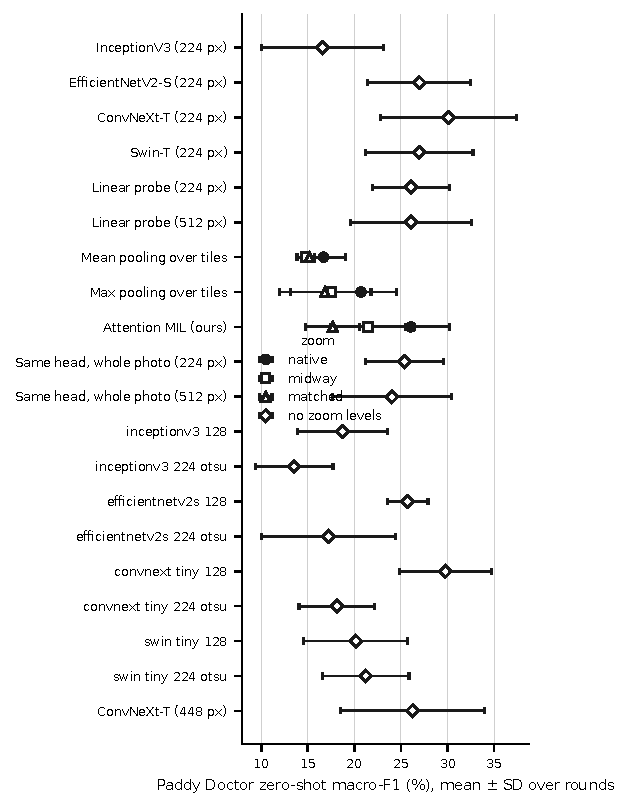
\includegraphics[width=0.8\columnwidth]{final_paddy_zoom.pdf}
\caption{Zero-shot macro-F1 (\%) on Paddy Doctor, mean $\pm$ SD over the 5 round-models, for every method and condition; the tile methods are shown at native, midway and matched zoom.}
\label{fig:paddy-zoom}
\end{figure}

On Paddy Doctor (native zoom, Table~\ref{tab:final_main}) Attention MIL scores 26.1 $\pm$ 4.2 macro-F1 and 33.8 $\pm$ 2.9
balanced accuracy, where 25.0 is chance for balanced accuracy. Every method, including the 128-px and Otsu conditions, falls
between 13.5 and 30.1 macro-F1; ConvNeXt-T at 224 px is highest (30.1 $\pm$ 7.3). By the rule declared before the run, H3 holds if
Attention MIL beats each of the four fine-tuned 224-px models; it beats only InceptionV3 (+13.9), so \textbf{H3 is not
shown}. Pooling the five round-models of each method, EfficientNetV2-S and ConvNeXt-T at 224 px scored higher than Attention MIL
(by 3.8 and 4.3 points; their ranges lie entirely below zero), but the declared rule asks for one direction only and calls
these ``no clear difference''. Many models predict almost one class for every field photo: pooled over its five
round-models, Attention MIL recalls 79.2\,\% of leaf-blast photos but 0.1\,\% of healthy photos. Matching the zoom did not help the tile methods:
Attention MIL scores 21.5 at midway and 17.7 at matched zoom (Table~\ref{tab:final_main}; Fig.~\ref{fig:paddy-zoom}).

\subsection{Do the heat maps point at symptoms (H4)?}
\PaperTable[\SmallWide]{explain}{Deletion test on the session-blocked test photos (seed-0 models): macro-F1 (\%) after removing the $k$ most-attended tiles or $k$ random tiles, and the true-class probability gap (random minus top-$k$ removed, points) with 95\,\% photo and block ranges and rounds won.}

\PaperTable[\SmallWide]{explain_ratings}{Blind ratings of 50 heat maps (validation photos) by two independent sets of three model raters: share of each answer to ``does the hot area cover visible symptoms?'', share of maps on which all three raters agree, and Fleiss' $\kappa$.}

\begin{figure*}[t]
\centering
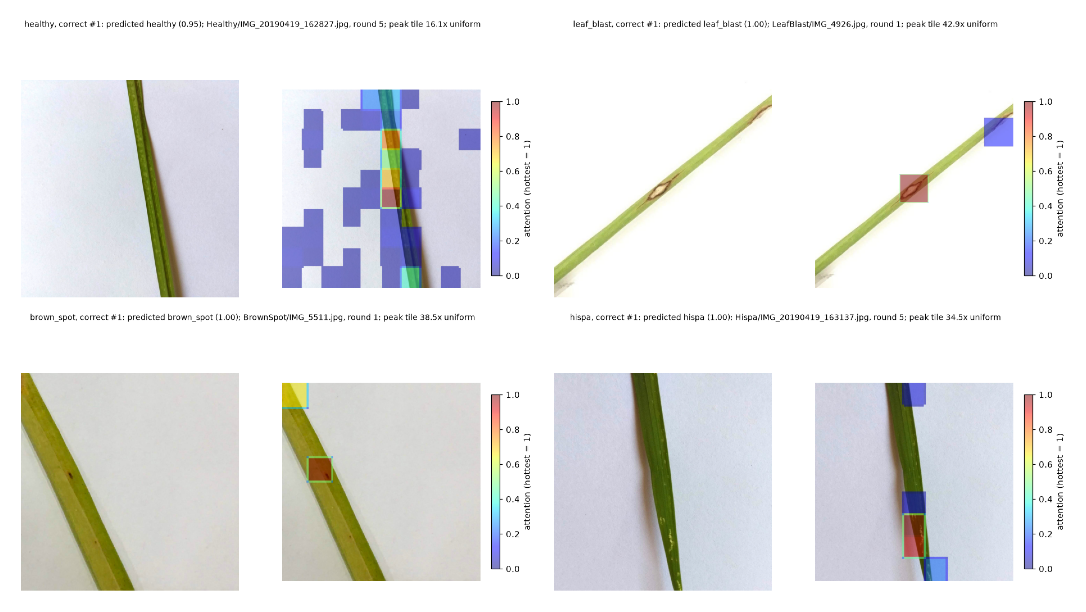
\includegraphics[width=0.7\textwidth]{final_heatmaps.pdf}
\caption{Heat maps for the most confident correct validation photo of each class (photo and attention overlay). These are the best case of each class, not typical examples; colour is attention relative to the photo's maximum and not a disease probability.}
\label{fig:heatmaps}
\end{figure*}

In the deletion test, in the spirit of RISE \cite{petsiuk2018rise}, we removed the $k$ most-attended tiles or $k$ random tiles from each test photo and rescored it
(Table~\ref{tab:final_explain}). Removing 16 attended tiles lowers macro-F1 from 77.9 to 15.6, while removing 16 random
tiles lowers it only to 75.3. The true-class probability falls 25.4 points more after the attended tiles are removed
(photo range $[24.5, 26.2]$, block range $[18.2, 32.8]$, 5 of 5 rounds), and the gap grows with $k$. It is negative for
healthy photos ($-12.9$ at $k=16$), which have no symptom to find. On Paddy Doctor photos the effect is small (2.2 points
at $k=16$, photo range only). On the test photos Attention MIL puts 15.3\,\% of its attention on background tiles, which are
74.5\,\% of all tiles; on Paddy Doctor photos attention on background (20.3\,\%) is no different from the tile share (19.7\,\%).
Two independent sets of three disclosed model raters rated 50 blind heat maps of validation photos
(Fig.~\ref{fig:heatmaps}, Table~\ref{tab:final_explain-ratings}): the hot area covers visible symptoms for 39.3\,\% (set 1)
and 49.3\,\% (set 2) of the ratings, partly for 32.0 and 24.0\,\%, and not for 28.7 and 26.7\,\%. Fleiss' $\kappa$
\cite{fleiss1971kappa} is 0.88 and 0.75, and the majority answers of the two sets agree on 84.0\,\% of the maps. The
heat maps are qualitative evidence of where the head looks; they carry no severity claim.

\subsection{Cost (H5)}
\PaperTable[\WideLayout]{cost}{Parameters (M), disk size (MB), training cache (GB), time per photo (s) on GPU and CPU, peak GPU and CPU memory (MB) and test macro-F1 (\%). Times are medians over 100 photos, one at a time from disk, decoding included, on one machine (RTX 4060, Ryzen 7 7700) and depend on it.}

\begin{figure}[t]
\centering
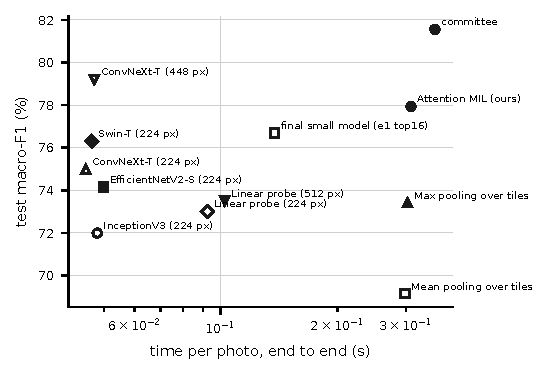
\includegraphics[width=\columnwidth]{final_cost.pdf}
\caption{Test macro-F1 (\%) against time per photo, end to end (log scale), session-blocked split; one machine (RTX 4060 GPU).}
\label{fig:cost}
\end{figure}

Table~\ref{tab:final_cost} and Fig.~\ref{fig:cost} give the cost. Attention MIL needs about 79 encoder passes per photo, so it takes 0.31 s per
photo on the GPU and 5.36 s on the CPU, about 80 times the 224-px whole-image models on the CPU (0.06--0.07 s); the head is small, but the frozen encoder must run for every tile. Compression variants were scored on validation photos
(reference 78.5, 5.36 s on the CPU): keeping 16 tiles gave 76.5 at 1.21 s; a head distilled from the smaller DINOv3
ViT-S/16 gave 78.6; 8-bit linear layers failed (23.6); and the 16-tile model exported to ONNX took 0.93 s on the CPU. The
Small model (16 tiles) was tested once and scores 76.7 on test, with no clear difference from Attention MIL ($+1.4$, 3 of 5
rounds). No rule for H5 was declared, so this is a descriptive answer; times are from one machine and depend on its hardware.

\subsection{Partition order}
\begin{figure}[t]
\centering
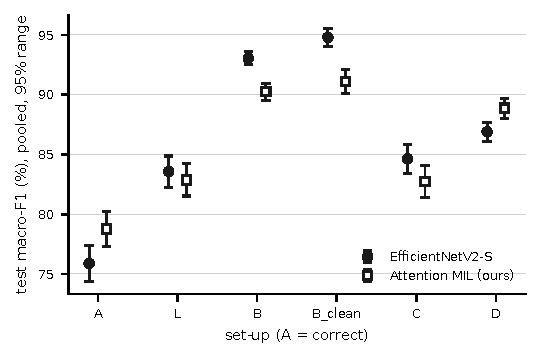
\includegraphics[width=\columnwidth]{final_partition_order.pdf}
\caption{Partition-order experiment: pooled test macro-F1 (\%) with 95\,\% ranges. A: session-blocked split, augmentation on training photos only (correct); L: locked split; B: augment first, then split the copies at random; B\_clean: B scored on clean copies only; C: random split without grouping; D: train and score on the same photos. Full table in Table~\ref{tab:final_partition-order}.}
\label{fig:partition-order}
\end{figure}

Fig.~\ref{fig:partition-order} shows how much three faulty set-ups raise the score of two models trained under the
correct protocol (A). The set-ups are deliberately wrong and are not estimates of performance. Augmenting every photo eight
times and then splitting the copies at random (B) raises macro-F1 by 17.2 points for EfficientNetV2-S and 11.5 for Attention MIL
(pooled scores, both clearly above A). Splitting photos at random without grouping (C) raises it by 8.8 and 4.0, and
training and scoring on the same photos (D) by 11.0 and 10.1. The locked split (L) is 7.7 and 4.1 points above A. The
pattern holds for both models, so the order of splitting and augmenting changes a score by more than most differences
between methods in this field.
